\documentclass[xetex,mathserif,serif]{beamer}
\usepackage{polyglossia}
\setdefaultlanguage[babelshorthands=true]{russian}
\usepackage{minted}
\usepackage{tabu}
\usepackage{moresize}

\useoutertheme{infolines}

\usepackage{fontspec}
\setmainfont{FreeSans}
\newfontfamily{\russianfonttt}{FreeSans}

\definecolor{links}{HTML}{2A1B81}
\hypersetup{colorlinks,linkcolor=,urlcolor=links}

\setbeamertemplate{blocks}[rounded][shadow=false]

\setbeamercolor*{block title alerted}{fg=red!50!black,bg=red!20}
\setbeamercolor*{block body alerted}{fg=black,bg=red!10}

\tabulinesep=1.2mm

\title{Базы данных и Java}
\author[Юрий Литвинов]{Юрий Литвинов\\\small{\textcolor{gray}{yurii.litvinov@gmail.com}}}
\date{13.02.2019г}

\newcommand{\attribution}[1] {
\vspace{-5mm}\begin{flushright}\begin{scriptsize}\textcolor{gray}{\textcopyright\, #1}\end{scriptsize}\end{flushright}
}

\begin{document}

	\frame{\titlepage}

	\section{Введение}

	\begin{frame}
		\frametitle{СУБД}
		\begin{itemize}
			\item Реляционные
			\begin{itemize}
				\item Отношения
				\item Операции
			\end{itemize}
			\item Объектно-ориентированные
			\begin{itemize}
				\item Сериализованные объекты
			\end{itemize}
			\item Иерархические
			\item ...
		\end{itemize}
	\end{frame}

	\begin{frame}
		\frametitle{Реляционные vs ОО-СУБД}
		\begin{itemize}
			\item Реляционные
			\begin{itemize}
				\item Сложность интеграции с ОО-кодом
				\begin{itemize}
					\item ORM (Microsoft Entity Framework, Hibernate, MyBatis, ...)
				\end{itemize}
				\item Эффективные и выразительные запросы
			\end{itemize}
			\item Объектно-ориентированные
			\begin{itemize}
				\item Проще, легковеснее, не требуют ORM
				\item ``Бедный'' язык запросов
				\item Часто не умеют того, что для реляционных СУБД естественно (например, транзакций)
			\end{itemize}
		\end{itemize}
	\end{frame}

	\section{Реляционная модель данных}

	\begin{frame}
		\frametitle{Реляционная модель данных}
		\begin{center}
			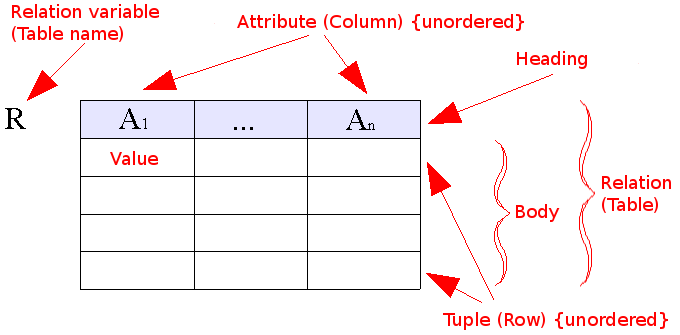
\includegraphics[width=0.9\textwidth]{relationalModel.png}
			\attribution{Wikipedia}
		\end{center}
	\end{frame}

	\begin{frame}
		\frametitle{Пример таблицы}
		\begin{center}
			\begin{tabu} {| X[0.9 l p] | X[1 l p] | X[1 l p] | X[1 l p] |}
				\tabucline-
				CustomerID       & TaxID        & Name       & Address           \\
				\tabucline-
				\everyrow{\tabucline-}
				1234567890       & 555-5512222  & Munmun     & 323 Broadway      \\
				2223344556       & 555-5523232  & Wile E.    & 1200 Main Street  \\
				3334445563       & 555-5533323  & Ekta       & 871 1st Street    \\
				423242432        & 555-5325523  & E.F. Codd  & 123 It Way        \\
			\end{tabu}
		\end{center}
	\end{frame}

	\begin{frame}
		\frametitle{Ключи}
		\begin{columns}
			\begin{column}{0.5\textwidth}
			\begin{itemize}
				\item Первичные (primary)
				\begin{itemize}
					\item Естественные
					\begin{itemize}
						\item Составные
					\end{itemize}
					\item Суррогатные
				\end{itemize}
				\item Внешние (foreign)
			\end{itemize}
			\end{column}
			\begin{column}{0.5\textwidth}
				\begin{scriptsize}
					CITY
					\begin{tabu} {| X[0.2 l p] | X[1 l p] |}
						\tabucline-
						ID      & Name \\
						\tabucline-
						\everyrow{\tabucline-}
						1       & Москва \\
						2       & Санкт-Петербург \\
						3       & Владивосток \\
					\end{tabu}
					\vspace{3mm}
					STREET
					\begin{tabu} {| X[0.2 l p] | X[1 l p] | X[0.7 l p] |}
						\tabucline-
						ID       & Name             & ID\_CITY \\
						\tabucline-
						\everyrow{\tabucline-}
						181      & Малая Бронная    & 1 \\
						182      & Тверской Бульвар & 1 \\
						183      & Невский проспект & 2 \\
						184      & Пушкинская       & 2 \\
						185      & Светланская      & 3 \\
						186      & Пушкинская       & 3 \\
					\end{tabu}
				\end{scriptsize}
			\end{column}
		\end{columns}
	\end{frame}

	\begin{frame}
		\frametitle{Ограничения}
		\begin{itemize}
			\item PRIMARY KEY
			\item FOREIGN KEY
			\item NOT NULL
			\item UNIQUE
			\item ...
		\end{itemize}
	\end{frame}

	\begin{frame}
		\frametitle{SQL SELECT}
		\begin{center}
			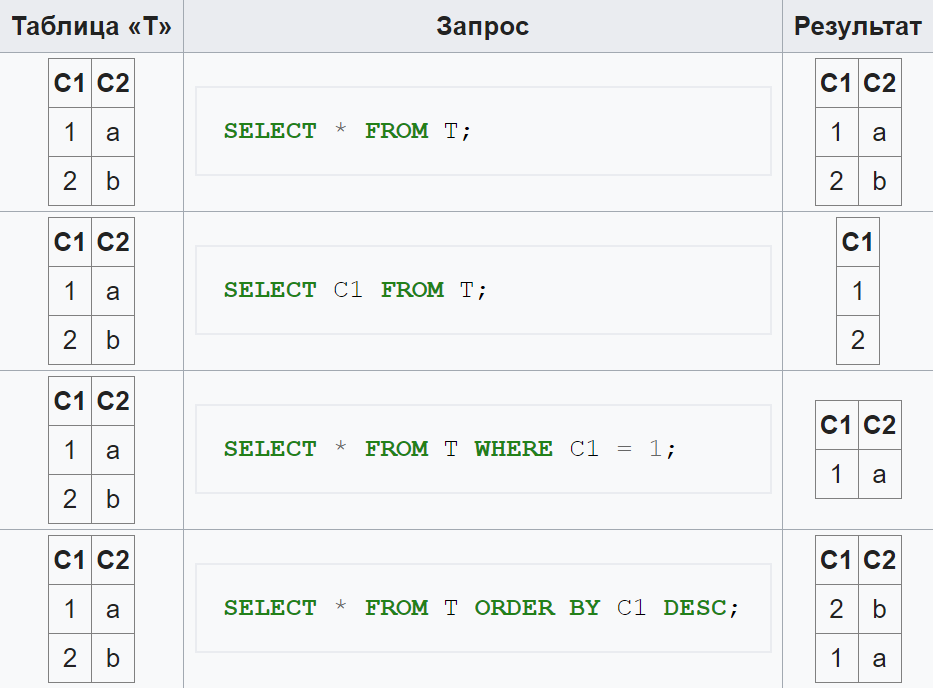
\includegraphics[width=0.7\textwidth]{select.png}
			\attribution{Wikipedia}
		\end{center}
	\end{frame}

	\begin{frame}[fragile]
		\frametitle{SELECT, вложенные запросы}
		\begin{minted}{sql}
SELECT isbn,
       title,
       price
FROM Book
WHERE price < (SELECT AVG(price) FROM Book)
ORDER BY title;
		\end{minted}
	\end{frame}

	\begin{frame}
		\frametitle{INNER JOIN}
		\begin{center}
			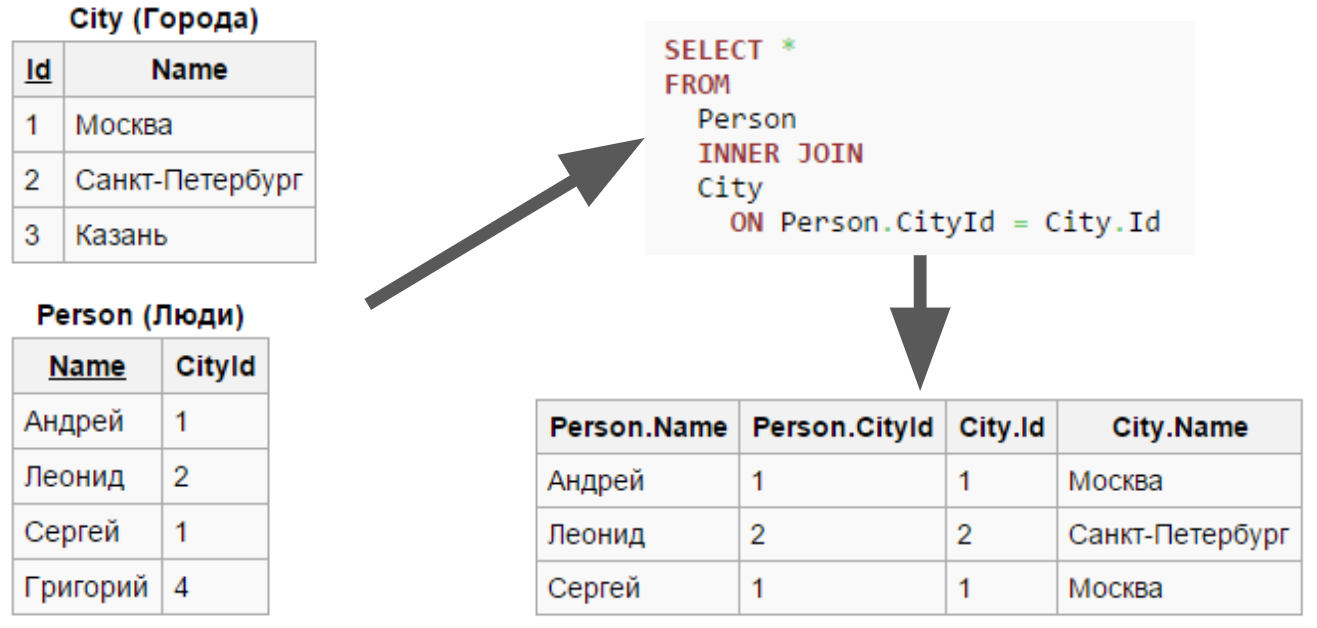
\includegraphics[width=0.9\textwidth]{innerJoin.png}
			\attribution{Wikipedia}
		\end{center}
	\end{frame}

	\begin{frame}
		\frametitle{OUTER JOIN}
		\begin{center}
			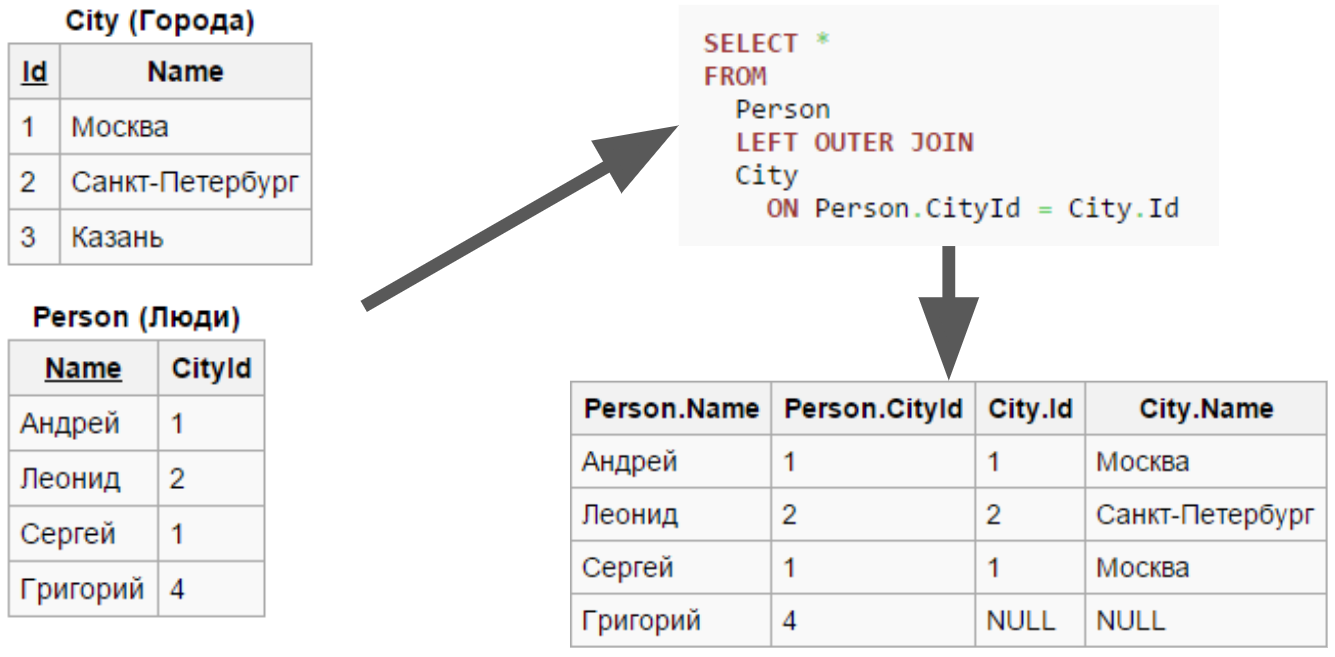
\includegraphics[width=0.9\textwidth]{outerJoin.png}
			\attribution{Wikipedia}
		\end{center}
	\end{frame}

	\begin{frame}
		\frametitle{CROSS JOIN}
		\begin{center}
			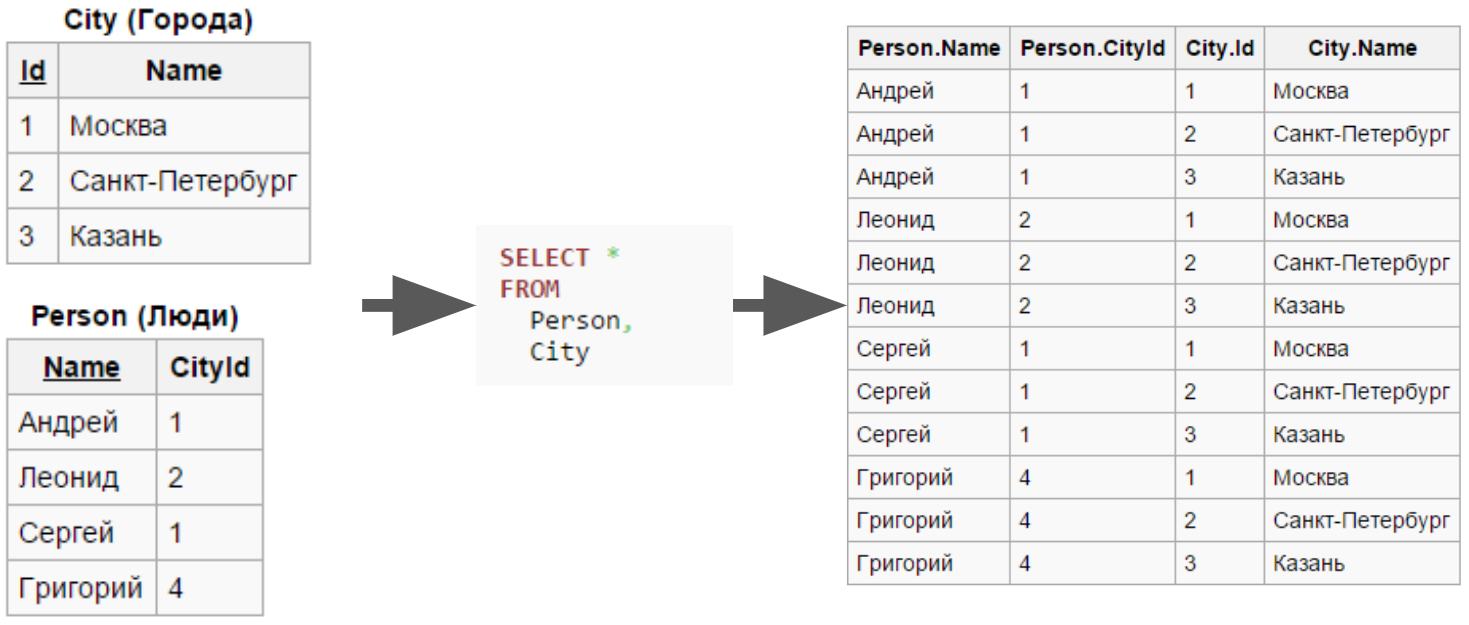
\includegraphics[width=0.9\textwidth]{crossJoin.png}
			\attribution{Wikipedia}
		\end{center}
	\end{frame}

	\begin{frame}[fragile]
		\frametitle{INSERT, UPDATE, DELETE}
		\begin{small}
			INSERT:
			\begin{minted}{sql}
INSERT INTO phone_books VALUES ('Peter Doe', '555-2323');
			\end{minted}

			\vspace{3mm}
			UPDATE:
			\begin{minted}{sql}
UPDATE persons SET
        street = 'Nissestien 67',
        city = 'Sandnes',
    WHERE lastname = 'Tjessem' AND firstname = 'Jakob';
			\end{minted}

			\vspace{3mm}
			DELETE:
			\begin{minted}{sql}
DELETE ab, b
    FROM Authors AS a, AuthorArticle AS ab, Articles AS b
    WHERE a.AuthID = ab.AuthID AND ab.ArticleID = b.ArticleID
        AND AuthorLastName = 'Henry';
			\end{minted}
		\end{small}
	\end{frame}

	\begin{frame}[fragile]
		\frametitle{Работа с метаинформацией}
		\begin{small}
			CREATE TABLE:
			\begin{minted}{sql}
CREATE TABLE Students (
    Code INTEGER NOT NULL,
    Name NCHAR(30) NOT NULL,
    Address NVARCHAR(50),
    Mark DECIMAL);
			\end{minted}

			\vspace{3mm}
			DROP TABLE:
			\begin{minted}{sql}
DROP TABLE Students;
			\end{minted}
		\end{small}

		\begin{center}
			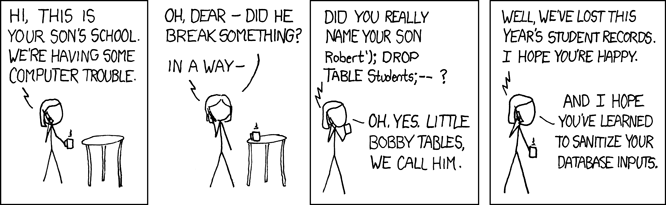
\includegraphics[width=0.7\textwidth]{bobbyTables.png}
			\attribution{XKCD}
		\end{center}
	\end{frame}

	\begin{frame}[fragile]
		\frametitle{Работа с метаинформацией}
		ALTER TABLE:
		\begin{minted}{sql}
ALTER TABLE Students ADD email VARCHAR(MAX);
ALTER TABLE Students DROP COLUMN email;

ALTER TABLE Students ADD PRIMARY KEY (Code);

		\end{minted}
	\end{frame}

	\begin{frame}[fragile]
		\frametitle{Низкоуровневый API: JDBC}
		\begin{itemize}
			\item API для доступа к реляционным базам данных из программ на Java
			\item Позволяет выполнять SQL-запросы
			\item Пример:
			\begin{footnotesize}
				\begin{minted}{java}
try (Connection conn = DriverManager.getConnection(
    "jdbc:mariadb://localhost:3306/mydb",
    "root",
    "1")) {
        try (Statement stmt = conn.createStatement()) {
            stmt.executeUpdate(
                "INSERT INTO cities(Name) VALUES ('St. Petersburg')" );
        }
    }
				\end{minted}
			\end{footnotesize}
		\end{itemize}
	\end{frame}

	\begin{frame}[fragile]
		\frametitle{JDBC: Пример запроса к базе}
		\begin{footnotesize}
			\begin{minted}{java}
try (Statement stmt = conn.createStatement();
    ResultSet rs = stmt.executeQuery("SELECT * FROM Cities")
) {
    while (rs.next()) {
        int numColumns = rs.getMetaData().getColumnCount();
        for (int i = 1 ; i <= numColumns ; i++) {
            System.out.println("COLUMN " + i + " = " + rs.getObject(i));
        }
    }
}
			\end{minted}
		\end{footnotesize}
	\end{frame}

	\begin{frame}
		\frametitle{SQLite}
		\begin{itemize}
			\item База данных, работающая в пространстве процесса
			\begin{itemize}
				\item Не требует отдельного сервера, поставляется как .jar-ник
				\item Не требует администрирования и настройки
			\end{itemize}
			\item Альтернатива хранению данных в файлах
			\item Умеет полноценные SQL-запросы
			\begin{itemize}
				\item Зато плоха в обработке больших объёмов данных или когда нагрузка слишком большая
				\item Не умеет ``из коробки'' работать по сети
			\end{itemize}
			\item Хранит всю базу в одном файле
			\item Размер библиотеки и используемая память могут быть очень маленькими
			\begin{itemize}
				\item Хороша для встроенных устройств
			\end{itemize}
		\end{itemize}
	\end{frame}

	\begin{frame}[fragile]
		\frametitle{SQLite, пример}
		\begin{footnotesize}
			\begin{minted}{java}
try (Connection conn = DriverManager.getConnection(
    "jdbc:sqlite:sample.db")) {
    try (Statement stmt = conn.createStatement()) {
        stmt.executeUpdate("drop table if exists cities");
        stmt.executeUpdate("create table cities (id integer, name varchar(50))");
        stmt.executeUpdate("insert into cities values(1, 'St. Petersburg')");
        stmt.executeUpdate("insert into cities values(2, 'Moscow')");
        try (ResultSet rs = stmt.executeQuery("select * from cities")) {
            while (rs.next()) {
                // read the result set
                System.out.println("name = " + rs.getString("name"));
                System.out.println("id = " + rs.getInt("id"));
            }
        }
    }
}
			\end{minted}
		\end{footnotesize}
	\end{frame}

	\begin{frame}
		\frametitle{ORM-системы, Hibernate}
		\begin{columns}
			\begin{column}{0.75\textwidth}
				\begin{itemize}
					\item Умеет генерировать прокси-объекты, которые можно использовать в приложении для работы с таблицами БД
					\item Основные классы:
					\begin{itemize}
						\item Configuration --- хранит конфигурацию, в частности, к чему и как подключаться, умеет создавать SessionFactory
						\item SessionFactory --- представляет отображение таблиц БД на классы из Data Access Layer, создаёт объекты Session, одна на приложение
						\item Session --- ``Единица работы'', штука, которая реально связывается с БД и обновляет её таблицы результатами изменений в DAL
						\item Transaction --- транзакция (атомарная операция) в БД. Сессия создаёт транзакции, но может иметь только одну открытую транзакцию в каждый момент
					\end{itemize}
				\end{itemize}
			\end{column}
			\begin{column}{0.25\textwidth}
				\begin{center}
					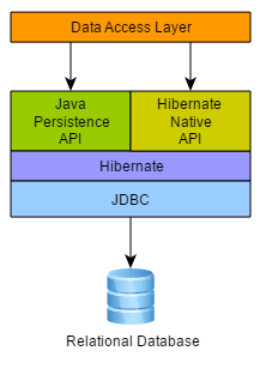
\includegraphics[width=0.9\textwidth]{hibernate.png}
				\end{center}
			\end{column}
		\end{columns}
	\end{frame}

	\begin{frame}
		\frametitle{NoSQL, MongoDB}
		\begin{itemize}
			\item Документо-ориентированная СУБД
			\begin{itemize}
				\item Единица хранения --- документ
				\item Набор пар ``имя''-``значение'', значение может быть сложного типа
				\item Коллекция --- список документов
			\end{itemize}
			\item Сервер --- отдельный процесс
			\begin{itemize}
				\item Впрочем, не требует особого администрирования
			\end{itemize}
			\item Morphia --- типобезопасный API для работы с базой поверх mongodb-driver
			\item Не использует JDBC
			\item Использует разумные умолчания --- если БД или коллекции при первом обращении нет, она будет создана
		\end{itemize}
	\end{frame}

	\begin{frame}[fragile]
		\frametitle{Пример аннотированного объекта}
		\begin{footnotesize}
			\begin{minted}{java}
@Entity
public class City {
    @Id private int id;
    private String name;

    public City() { }
    public City(String name) {
        this.name = name;
    }

    public String getName() {
        return name;
    }
}
			\end{minted}
		\end{footnotesize}
	\end{frame}

	\begin{frame}[fragile]
		\frametitle{Пример добавления в базу}
		\begin{footnotesize}
			\begin{minted}{java}
final Morphia morphia = new Morphia();
morphia.mapPackage("com.example");
final Datastore datastore = morphia.createDatastore(new MongoClient(), "mydb");

City stPetersburg = new City("St. Petersburg");
datastore.save(stPetersburg);
			\end{minted}
		\end{footnotesize}
	\end{frame}

	\begin{frame}[fragile]
		\frametitle{Пример чтения из базы}
		\begin{footnotesize}
			\begin{minted}{java}
final Morphia morphia = new Morphia();
morphia.mapPackage("com.example");
final Datastore datastore = morphia.createDatastore(new MongoClient(), "mydb");

for (City city : datastore.find(City.class)) {
    System.out.println(city.getName());
}
			\end{minted}
		\end{footnotesize}
	\end{frame}

\end{document}
